\documentclass[twoside]{book}

% Packages required by doxygen
\usepackage{fixltx2e}
\usepackage{calc}
\usepackage{doxygen}
\usepackage[export]{adjustbox} % also loads graphicx
\usepackage{graphicx}
\usepackage[utf8]{inputenc}
\usepackage{makeidx}
\usepackage{multicol}
\usepackage{multirow}
\PassOptionsToPackage{warn}{textcomp}
\usepackage{textcomp}
\usepackage[nointegrals]{wasysym}
\usepackage[table]{xcolor}

% Font selection
\usepackage[T1]{fontenc}
\usepackage[scaled=.90]{helvet}
\usepackage{courier}
\usepackage{amssymb}
\usepackage{sectsty}
\renewcommand{\familydefault}{\sfdefault}
\allsectionsfont{%
  \fontseries{bc}\selectfont%
  \color{darkgray}%
}
\renewcommand{\DoxyLabelFont}{%
  \fontseries{bc}\selectfont%
  \color{darkgray}%
}
\newcommand{\+}{\discretionary{\mbox{\scriptsize$\hookleftarrow$}}{}{}}

% Page & text layout
\usepackage{geometry}
\geometry{%
  a4paper,%
  top=2.5cm,%
  bottom=2.5cm,%
  left=2.5cm,%
  right=2.5cm%
}
\tolerance=750
\hfuzz=15pt
\hbadness=750
\setlength{\emergencystretch}{15pt}
\setlength{\parindent}{0cm}
\setlength{\parskip}{3ex plus 2ex minus 2ex}
\makeatletter
\renewcommand{\paragraph}{%
  \@startsection{paragraph}{4}{0ex}{-1.0ex}{1.0ex}{%
    \normalfont\normalsize\bfseries\SS@parafont%
  }%
}
\renewcommand{\subparagraph}{%
  \@startsection{subparagraph}{5}{0ex}{-1.0ex}{1.0ex}{%
    \normalfont\normalsize\bfseries\SS@subparafont%
  }%
}
\makeatother

% Headers & footers
\usepackage{fancyhdr}
\pagestyle{fancyplain}
\fancyhead[LE]{\fancyplain{}{\bfseries\thepage}}
\fancyhead[CE]{\fancyplain{}{}}
\fancyhead[RE]{\fancyplain{}{\bfseries\leftmark}}
\fancyhead[LO]{\fancyplain{}{\bfseries\rightmark}}
\fancyhead[CO]{\fancyplain{}{}}
\fancyhead[RO]{\fancyplain{}{\bfseries\thepage}}
\fancyfoot[LE]{\fancyplain{}{}}
\fancyfoot[CE]{\fancyplain{}{}}
\fancyfoot[RE]{\fancyplain{}{\bfseries\scriptsize Generated by Doxygen }}
\fancyfoot[LO]{\fancyplain{}{\bfseries\scriptsize Generated by Doxygen }}
\fancyfoot[CO]{\fancyplain{}{}}
\fancyfoot[RO]{\fancyplain{}{}}
\renewcommand{\footrulewidth}{0.4pt}
\renewcommand{\chaptermark}[1]{%
  \markboth{#1}{}%
}
\renewcommand{\sectionmark}[1]{%
  \markright{\thesection\ #1}%
}

% Indices & bibliography
\usepackage{natbib}
\usepackage[titles]{tocloft}
\setcounter{tocdepth}{3}
\setcounter{secnumdepth}{5}
\makeindex

% Hyperlinks (required, but should be loaded last)
\usepackage{ifpdf}
\ifpdf
  \usepackage[pdftex,pagebackref=true]{hyperref}
\else
  \usepackage[ps2pdf,pagebackref=true]{hyperref}
\fi
\hypersetup{%
  colorlinks=true,%
  linkcolor=blue,%
  citecolor=blue,%
  unicode%
}

% Custom commands
\newcommand{\clearemptydoublepage}{%
  \newpage{\pagestyle{empty}\cleardoublepage}%
}

\usepackage{caption}
\captionsetup{labelsep=space,justification=centering,font={bf},singlelinecheck=off,skip=4pt,position=top}

%===== C O N T E N T S =====

\begin{document}

% Titlepage & ToC
\hypersetup{pageanchor=false,
             bookmarksnumbered=true,
             pdfencoding=unicode
            }
\pagenumbering{alph}
\begin{titlepage}
\vspace*{7cm}
\begin{center}%
{\Large Timers and Motor Cont \\[1ex]\large Lab05 }\\
\vspace*{1cm}
{\large Generated by Doxygen 1.8.13}\\
\end{center}
\end{titlepage}
\clearemptydoublepage
\pagenumbering{roman}
\tableofcontents
\clearemptydoublepage
\pagenumbering{arabic}
\hypersetup{pageanchor=true}

%--- Begin generated contents ---
\chapter{Main Page}
\label{index}\hypertarget{index}{}\hypertarget{index_Introduction}{}\section{Introduction}\label{index_Introduction}
This will serve as documentation for lab 5 for the C\+E\+N\+G447\+: Embedded systems classes for the Spring of 2019.

Lab 5\textquotesingle{}s goal was use Timer0 to generate a P\+WM signal to run the motors on the Elegoo robot using the L\+M298 motor controller module and the provided header file. The source code can be found \href{https://github.com/warlock31415/Embedded-CENG447/tree/u
            se_classes/Lab05}{\tt here}

The clock is set according to the following table\+: \tabulinesep=1mm
\begin{longtabu} spread 0pt [c]{*{2}{|X[-1]}|}
\hline
\rowcolor{\tableheadbgcolor}\textbf{ Set \# }&\textbf{ Prescaler  }\\\cline{1-2}
\endfirsthead
\hline
\endfoot
\hline
\rowcolor{\tableheadbgcolor}\textbf{ Set \# }&\textbf{ Prescaler  }\\\cline{1-2}
\endhead
0 &No clock source \\\cline{1-2}
1 &No prescaler \\\cline{1-2}
2 &clk/8 \\\cline{1-2}
3 &clk/64 \\\cline{1-2}
4 &clk/256 \\\cline{1-2}
5 &clk/1024 \\\cline{1-2}
6 &Ext clk on T0 pin. Clock on falling edge \\\cline{1-2}
7 &Ext clk on T0 pin. Clock on rising edge \\\cline{1-2}
\end{longtabu}
The set \# is passed into the init member function. This sets the frequency of the P\+WM according to the table above.\hypertarget{index_Video}{}\section{Video}\label{index_Video}
Please follow \href{https://youtu.be/2wUh4nnQhK4}{\tt this link}\hypertarget{index_Document}{}\section{Document}\label{index_Document}
Download the P\+DF by clicking \href{./Lab4.pdf}{\tt here}\hypertarget{index_Issues}{}\section{Issues}\label{index_Issues}

\begin{DoxyEnumerate}
\item Half power
\begin{DoxyItemize}
\item Since two motors are connected to the same output on the motor controller output, the motors only get half the power each thus are never at full output.
\end{DoxyItemize}
\item Incorrect frequency
\begin{DoxyItemize}
\item The motors make a whiney noise if too high of a frequency or too low a frequency is supplied 
\end{DoxyItemize}
\end{DoxyEnumerate}
\chapter{Data Structure Index}
\section{Data Structures}
Here are the data structures with brief descriptions\+:\begin{DoxyCompactList}
\item\contentsline{section}{\hyperlink{classL298}{L298} }{\pageref{classL298}}{}
\end{DoxyCompactList}

\chapter{File Index}
\section{File List}
Here is a list of all documented files with brief descriptions\+:\begin{DoxyCompactList}
\item\contentsline{section}{\hyperlink{L298_8c}{L298.\+c} \\*This file contains functions for using the \hyperlink{classL298}{L298} motor driver }{\pageref{L298_8c}}{}
\item\contentsline{section}{\hyperlink{L298_8h}{L298.\+h} \\*This file contains functions declarations for using the \hyperlink{classL298}{L298} motor driver }{\pageref{L298_8h}}{}
\item\contentsline{section}{\hyperlink{main_8c}{main.\+c} \\*This is the main file for Lab 5. It declares the motor object and calls the appropriate functions to complete the required task }{\pageref{main_8c}}{}
\item\contentsline{section}{\hyperlink{pin__map_8h}{pin\+\_\+map.\+h} \\*This file contains functions declarations for using the \hyperlink{classL298}{L298} motor driver }{\pageref{pin__map_8h}}{}
\end{DoxyCompactList}

\chapter{Data Structure Documentation}
\hypertarget{classL298}{}\section{L298 Class Reference}
\label{classL298}\index{L298@{L298}}
\subsection*{Public Member Functions}
\begin{DoxyCompactItemize}
\item 
void \hyperlink{classL298_a5f5692e1f1f2649ad5fe43c3ec90b700}{init} (char clk)
\item 
void \hyperlink{classL298_a96b6c3c4a52195343bc19d05aa1efffd}{turn\+\_\+right} (int speed)
\item 
void \hyperlink{classL298_a182d163bdcc06330ffae43b0f49e0742}{forward} (int speed)
\item 
void \hyperlink{classL298_a4d818ee6a1c166a3e00c9e0fd0cf0d59}{back} (int speed)
\item 
void \hyperlink{classL298_a430051b0786596aac92f747121e9535c}{turn\+\_\+left} (int speed)
\item 
void \hyperlink{classL298_a638f680cf5d6dfba25e42ba96e19bee6}{square\+\_\+turn} (int speed)
\item 
void \hyperlink{classL298_added600b7b9c0a46be3474fa7e8b890c}{circ} ()
\end{DoxyCompactItemize}
\subsection*{Private Member Functions}
\begin{DoxyCompactItemize}
\item 
char \hyperlink{classL298_a937f021c405806051271c7ca4ab81fe2}{map} (int d\+\_\+cyc)
\end{DoxyCompactItemize}


\subsection{Member Function Documentation}
\mbox{\Hypertarget{classL298_a4d818ee6a1c166a3e00c9e0fd0cf0d59}\label{classL298_a4d818ee6a1c166a3e00c9e0fd0cf0d59}} 
\index{L298@{L298}!back@{back}}
\index{back@{back}!L298@{L298}}
\subsubsection{\texorpdfstring{back()}{back()}}
{\footnotesize\ttfamily void L298\+::back (\begin{DoxyParamCaption}\item[{int}]{speed }\end{DoxyParamCaption})}

This function sets the direction of the motors such that the both run backwards. The function calls the {\itshape \hyperlink{classL298_a937f021c405806051271c7ca4ab81fe2}{map()}} such that a percentage is mapped to a 0-\/255 range. 
\begin{DoxyParams}[1]{Parameters}
\mbox{\tt in}  & {\em speed} & A percentage of max speed 0-\/100\% \\
\hline
\end{DoxyParams}
\begin{DoxyReturn}{Returns}
void 
\end{DoxyReturn}
\mbox{\Hypertarget{classL298_added600b7b9c0a46be3474fa7e8b890c}\label{classL298_added600b7b9c0a46be3474fa7e8b890c}} 
\index{L298@{L298}!circ@{circ}}
\index{circ@{circ}!L298@{L298}}
\subsubsection{\texorpdfstring{circ()}{circ()}}
{\footnotesize\ttfamily void L298\+::circ (\begin{DoxyParamCaption}{ }\end{DoxyParamCaption})}

Sets the right side speed a little faster than the left speed so that the robot traces a circle. The radius of the circle is a relationship of the difference between the wheel speeds. 
\begin{DoxyParams}[1]{Parameters}
\mbox{\tt in}  & {\em speed} & A percentage of max speed 0-\/100\% \\
\hline
\end{DoxyParams}
\begin{DoxyReturn}{Returns}
void 
\end{DoxyReturn}
\mbox{\Hypertarget{classL298_a182d163bdcc06330ffae43b0f49e0742}\label{classL298_a182d163bdcc06330ffae43b0f49e0742}} 
\index{L298@{L298}!forward@{forward}}
\index{forward@{forward}!L298@{L298}}
\subsubsection{\texorpdfstring{forward()}{forward()}}
{\footnotesize\ttfamily void L298\+::forward (\begin{DoxyParamCaption}\item[{int}]{speed }\end{DoxyParamCaption})}

This function sets the direction of the motors such that the both run forwards. The function calls the {\itshape \hyperlink{classL298_a937f021c405806051271c7ca4ab81fe2}{map()}} such that a percentage is mapped to a 0-\/255 range. 
\begin{DoxyParams}[1]{Parameters}
\mbox{\tt in}  & {\em speed} & A percentage of max speed 0-\/100\% \\
\hline
\end{DoxyParams}
\begin{DoxyReturn}{Returns}
void 
\end{DoxyReturn}
\mbox{\Hypertarget{classL298_a5f5692e1f1f2649ad5fe43c3ec90b700}\label{classL298_a5f5692e1f1f2649ad5fe43c3ec90b700}} 
\index{L298@{L298}!init@{init}}
\index{init@{init}!L298@{L298}}
\subsubsection{\texorpdfstring{init()}{init()}}
{\footnotesize\ttfamily void L298\+::init (\begin{DoxyParamCaption}\item[{char}]{clk }\end{DoxyParamCaption})}

This function initializes Timer0 by setting the compare match registers A and B to clear on compare match. Setting the Waveform generation mode bits 1 and 0 and the P\+WM clock frquency. This function also sets appropriate pins on P\+O\+R\+TD as output. \begin{DoxyReturn}{Returns}
void 
\end{DoxyReturn}
\mbox{\Hypertarget{classL298_a937f021c405806051271c7ca4ab81fe2}\label{classL298_a937f021c405806051271c7ca4ab81fe2}} 
\index{L298@{L298}!map@{map}}
\index{map@{map}!L298@{L298}}
\subsubsection{\texorpdfstring{map()}{map()}}
{\footnotesize\ttfamily char L298\+::map (\begin{DoxyParamCaption}\item[{int}]{duty\+\_\+cyc }\end{DoxyParamCaption})\hspace{0.3cm}{\ttfamily [private]}}

This is a private function which is only available to functions inside the class. It takes a percentage of speed as input 100 being max and 0 being the minimum and maps it from 0 to 255. 
\begin{DoxyParams}[1]{Parameters}
\mbox{\tt in}  & {\em duty\+\_\+cyc} & Percentage of max speed \\
\hline
\mbox{\tt out}  & {\em duty\+\_\+cyc$\ast$255/100} & \\
\hline
\end{DoxyParams}
\begin{DoxyReturn}{Returns}
void 
\end{DoxyReturn}
\mbox{\Hypertarget{classL298_a638f680cf5d6dfba25e42ba96e19bee6}\label{classL298_a638f680cf5d6dfba25e42ba96e19bee6}} 
\index{L298@{L298}!square\+\_\+turn@{square\+\_\+turn}}
\index{square\+\_\+turn@{square\+\_\+turn}!L298@{L298}}
\subsubsection{\texorpdfstring{square\+\_\+turn()}{square\_turn()}}
{\footnotesize\ttfamily void L298\+::square\+\_\+turn (\begin{DoxyParamCaption}\item[{int}]{speed }\end{DoxyParamCaption})}

Calls the {\itshape \hyperlink{classL298_a96b6c3c4a52195343bc19d05aa1efffd}{turn\+\_\+right()}} function 4 times such that the robot traces a square whose side length is as long as 3s in equivalent distance. The spedd is set to 0 at the end. 
\begin{DoxyParams}[1]{Parameters}
\mbox{\tt in}  & {\em speed} & A percentage of max speed 0-\/100\% \\
\hline
\end{DoxyParams}
\begin{DoxyReturn}{Returns}
void 
\end{DoxyReturn}
\mbox{\Hypertarget{classL298_a430051b0786596aac92f747121e9535c}\label{classL298_a430051b0786596aac92f747121e9535c}} 
\index{L298@{L298}!turn\+\_\+left@{turn\+\_\+left}}
\index{turn\+\_\+left@{turn\+\_\+left}!L298@{L298}}
\subsubsection{\texorpdfstring{turn\+\_\+left()}{turn\_left()}}
{\footnotesize\ttfamily void L298\+::turn\+\_\+left (\begin{DoxyParamCaption}\item[{int}]{speed }\end{DoxyParamCaption})}

This function sets the direction of the motors such that the right side motors turn forwards and the left side mmotors turn the opposite direction. The function calls the {\itshape \hyperlink{classL298_a937f021c405806051271c7ca4ab81fe2}{map()}} such that a percentage is mapped to a 0-\/255 range. 
\begin{DoxyParams}[1]{Parameters}
\mbox{\tt in}  & {\em speed} & A percentage of max speed 0-\/100\% \\
\hline
\end{DoxyParams}
\begin{DoxyReturn}{Returns}
void 
\end{DoxyReturn}
\mbox{\Hypertarget{classL298_a96b6c3c4a52195343bc19d05aa1efffd}\label{classL298_a96b6c3c4a52195343bc19d05aa1efffd}} 
\index{L298@{L298}!turn\+\_\+right@{turn\+\_\+right}}
\index{turn\+\_\+right@{turn\+\_\+right}!L298@{L298}}
\subsubsection{\texorpdfstring{turn\+\_\+right()}{turn\_right()}}
{\footnotesize\ttfamily void L298\+::turn\+\_\+right (\begin{DoxyParamCaption}\item[{int}]{speed }\end{DoxyParamCaption})}

This function sets the direction of the motors such that the left side motors turn forwards and the right side mmotors turn the opposite direction. The function calls the {\itshape \hyperlink{classL298_a937f021c405806051271c7ca4ab81fe2}{map()}} such that a percentage is mapped to a 0-\/255 range. 
\begin{DoxyParams}[1]{Parameters}
\mbox{\tt in}  & {\em speed} & A percentage of max speed 0-\/100\% \\
\hline
\end{DoxyParams}
\begin{DoxyReturn}{Returns}
void 
\end{DoxyReturn}


The documentation for this class was generated from the following files\+:\begin{DoxyCompactItemize}
\item 
\hyperlink{L298_8h}{L298.\+h}\item 
\hyperlink{L298_8c}{L298.\+c}\end{DoxyCompactItemize}

\chapter{File Documentation}
\hypertarget{L298_8c}{}\section{L298.\+c File Reference}
\label{L298_8c}\index{L298.\+c@{L298.\+c}}


This file contains functions for using the \hyperlink{classL298}{L298} motor driver.  


{\ttfamily \#include \char`\"{}L298.\+h\char`\"{}}\newline
{\ttfamily \#include \char`\"{}pin\+\_\+map.\+h\char`\"{}}\newline
{\ttfamily \#include $<$avr/io.\+h$>$}\newline
{\ttfamily \#include $<$util/delay.\+h$>$}\newline
Include dependency graph for L298.\+c\+:\nopagebreak
\begin{figure}[H]
\begin{center}
\leavevmode
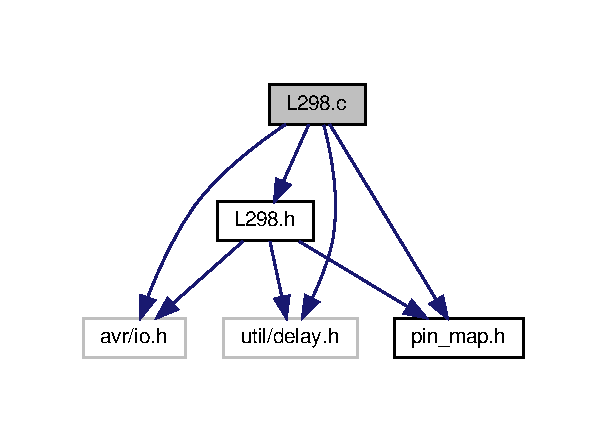
\includegraphics[width=292pt]{L298_8c__incl}
\end{center}
\end{figure}


\subsection{Detailed Description}
This file contains functions for using the \hyperlink{classL298}{L298} motor driver. 

\begin{DoxyAuthor}{Author}
Pratik Kunkolienker 
\end{DoxyAuthor}
\begin{DoxyDate}{Date}
27 March 2019 
\end{DoxyDate}

\hypertarget{L298_8h}{}\section{L298.\+h File Reference}
\label{L298_8h}\index{L298.\+h@{L298.\+h}}


This file contains functions declarations for using the \hyperlink{classL298}{L298} motor driver.  


{\ttfamily \#include $<$avr/io.\+h$>$}\newline
{\ttfamily \#include $<$util/delay.\+h$>$}\newline
{\ttfamily \#include \char`\"{}pin\+\_\+map.\+h\char`\"{}}\newline
Include dependency graph for L298.\+h\+:\nopagebreak
\begin{figure}[H]
\begin{center}
\leavevmode
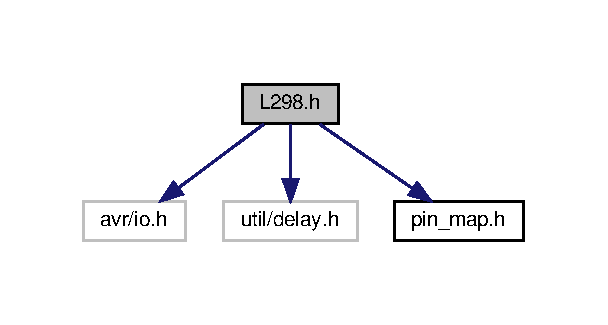
\includegraphics[width=292pt]{L298_8h__incl}
\end{center}
\end{figure}
This graph shows which files directly or indirectly include this file\+:\nopagebreak
\begin{figure}[H]
\begin{center}
\leavevmode
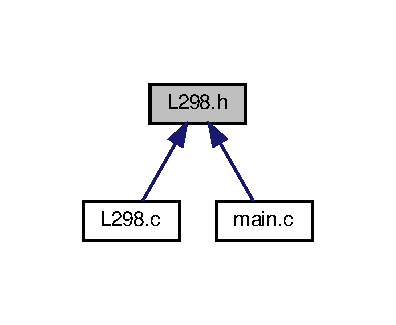
\includegraphics[width=190pt]{L298_8h__dep__incl}
\end{center}
\end{figure}
\subsection*{Data Structures}
\begin{DoxyCompactItemize}
\item 
class \hyperlink{classL298}{L298}
\end{DoxyCompactItemize}


\subsection{Detailed Description}
This file contains functions declarations for using the \hyperlink{classL298}{L298} motor driver. 

\begin{DoxyAuthor}{Author}
Pratik Kunkolienker 
\end{DoxyAuthor}
\begin{DoxyDate}{Date}
27 March 2019
\end{DoxyDate}
This file declares the \hyperlink{classL298}{L298} class and all the public and private functions. 
\hypertarget{main_8c}{}\section{main.\+c File Reference}
\label{main_8c}\index{main.\+c@{main.\+c}}


This is the main file for Lab 5. It declares the motor object and calls the appropriate functions to complete the required task.  


{\ttfamily \#include $<$avr/io.\+h$>$}\newline
{\ttfamily \#include $<$util/delay.\+h$>$}\newline
{\ttfamily \#include \char`\"{}L298.\+h\char`\"{}}\newline
Include dependency graph for main.\+c\+:\nopagebreak
\begin{figure}[H]
\begin{center}
\leavevmode
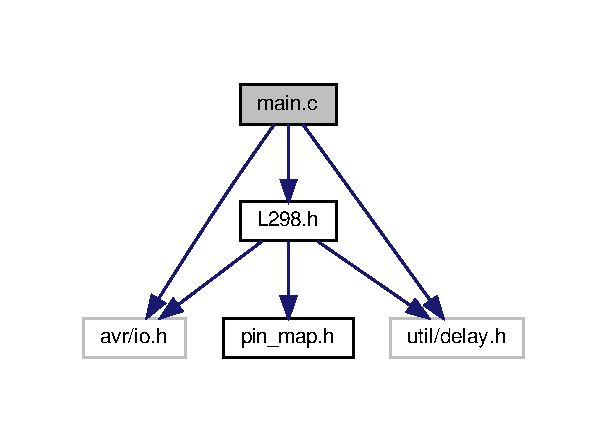
\includegraphics[width=292pt]{main_8c__incl}
\end{center}
\end{figure}
\subsection*{Macros}
\begin{DoxyCompactItemize}
\item 
\#define \hyperlink{main_8c_a734bbab06e1a9fd2e5522db0221ff6e3}{B\+A\+U\+D\+R\+A\+TE}~9600
\item 
\#define \hyperlink{main_8c_a0fac869d83ac1a584d6c45cf609f5fe7}{P\+R\+E\+S\+C\+A\+L\+ER}~F\+\_\+\+C\+PU/(\hyperlink{main_8c_a734bbab06e1a9fd2e5522db0221ff6e3}{B\+A\+U\+D\+R\+A\+TE}$\ast$16\+U\+L)-\/1
\end{DoxyCompactItemize}
\subsection*{Functions}
\begin{DoxyCompactItemize}
\item 
\mbox{\Hypertarget{main_8c_ae66f6b31b5ad750f1fe042a706a4e3d4}\label{main_8c_ae66f6b31b5ad750f1fe042a706a4e3d4}} 
int {\bfseries main} ()
\end{DoxyCompactItemize}
\subsection*{Variables}
\begin{DoxyCompactItemize}
\item 
\hyperlink{classL298}{L298} \hyperlink{main_8c_a6b41f9acb016dd748cdc43438c976163}{Motor}
\end{DoxyCompactItemize}


\subsection{Detailed Description}
This is the main file for Lab 5. It declares the motor object and calls the appropriate functions to complete the required task. 

\begin{DoxyAuthor}{Author}
Pratik Kunkolienker 
\end{DoxyAuthor}
\begin{DoxyDate}{Date}
27 March 2019
\end{DoxyDate}
This program was written has two versions. One compiled in C that uses functions. The other, compiled in C\+PP and uses classes. The main loop initializes the timer and calls the appropriate function such as circ and square turn. 

\subsection{Macro Definition Documentation}
\mbox{\Hypertarget{main_8c_a734bbab06e1a9fd2e5522db0221ff6e3}\label{main_8c_a734bbab06e1a9fd2e5522db0221ff6e3}} 
\index{main.\+c@{main.\+c}!B\+A\+U\+D\+R\+A\+TE@{B\+A\+U\+D\+R\+A\+TE}}
\index{B\+A\+U\+D\+R\+A\+TE@{B\+A\+U\+D\+R\+A\+TE}!main.\+c@{main.\+c}}
\subsubsection{\texorpdfstring{B\+A\+U\+D\+R\+A\+TE}{BAUDRATE}}
{\footnotesize\ttfamily \#define B\+A\+U\+D\+R\+A\+TE~9600}

U\+A\+RT baudrate \mbox{\Hypertarget{main_8c_a0fac869d83ac1a584d6c45cf609f5fe7}\label{main_8c_a0fac869d83ac1a584d6c45cf609f5fe7}} 
\index{main.\+c@{main.\+c}!P\+R\+E\+S\+C\+A\+L\+ER@{P\+R\+E\+S\+C\+A\+L\+ER}}
\index{P\+R\+E\+S\+C\+A\+L\+ER@{P\+R\+E\+S\+C\+A\+L\+ER}!main.\+c@{main.\+c}}
\subsubsection{\texorpdfstring{P\+R\+E\+S\+C\+A\+L\+ER}{PRESCALER}}
{\footnotesize\ttfamily \#define P\+R\+E\+S\+C\+A\+L\+ER~F\+\_\+\+C\+PU/(\hyperlink{main_8c_a734bbab06e1a9fd2e5522db0221ff6e3}{B\+A\+U\+D\+R\+A\+TE}$\ast$16\+U\+L)-\/1}

U\+A\+RT baudrate prescaler 

\subsection{Variable Documentation}
\mbox{\Hypertarget{main_8c_a6b41f9acb016dd748cdc43438c976163}\label{main_8c_a6b41f9acb016dd748cdc43438c976163}} 
\index{main.\+c@{main.\+c}!Motor@{Motor}}
\index{Motor@{Motor}!main.\+c@{main.\+c}}
\subsubsection{\texorpdfstring{Motor}{Motor}}
{\footnotesize\ttfamily \hyperlink{classL298}{L298} Motor}

Create a motor object that contains the initilization function and movement functions 
\hypertarget{pin__map_8h}{}\section{pin\+\_\+map.\+h File Reference}
\label{pin__map_8h}\index{pin\+\_\+map.\+h@{pin\+\_\+map.\+h}}


This file contains functions declarations for using the \hyperlink{classL298}{L298} motor driver.  


This graph shows which files directly or indirectly include this file\+:\nopagebreak
\begin{figure}[H]
\begin{center}
\leavevmode
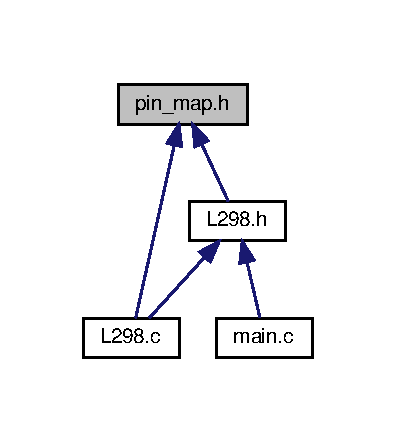
\includegraphics[width=190pt]{pin__map_8h__dep__incl}
\end{center}
\end{figure}
\subsection*{Macros}
\begin{DoxyCompactItemize}
\item 
\mbox{\Hypertarget{pin__map_8h_a2594694571481eade9f994c6c924be8f}\label{pin__map_8h_a2594694571481eade9f994c6c924be8f}} 
\#define \hyperlink{pin__map_8h_a2594694571481eade9f994c6c924be8f}{U\+S\+\_\+\+R\+E\+CV}~4
\begin{DoxyCompactList}\small\item\em Ultrasonic receive pin. \end{DoxyCompactList}\item 
\mbox{\Hypertarget{pin__map_8h_a60240f82bf58ebadfbe05d1762f6955b}\label{pin__map_8h_a60240f82bf58ebadfbe05d1762f6955b}} 
\#define \hyperlink{pin__map_8h_a60240f82bf58ebadfbe05d1762f6955b}{U\+S\+\_\+\+E\+C\+HO}~4
\begin{DoxyCompactList}\small\item\em Ultrasonic Echo pin. \end{DoxyCompactList}\item 
\mbox{\Hypertarget{pin__map_8h_a36c53a01b5fa0a07b02a673165abf62d}\label{pin__map_8h_a36c53a01b5fa0a07b02a673165abf62d}} 
\#define \hyperlink{pin__map_8h_a36c53a01b5fa0a07b02a673165abf62d}{U\+S\+\_\+\+T\+R\+IG}~5
\begin{DoxyCompactList}\small\item\em Iltrasonic trigger pin. \end{DoxyCompactList}\item 
\mbox{\Hypertarget{pin__map_8h_a4ecc92c13f887939fd27863acb00f4c2}\label{pin__map_8h_a4ecc92c13f887939fd27863acb00f4c2}} 
\#define \hyperlink{pin__map_8h_a4ecc92c13f887939fd27863acb00f4c2}{H\+\_\+\+A\+\_\+\+EN}~5
\begin{DoxyCompactList}\small\item\em H bridge motor enable A. \end{DoxyCompactList}\item 
\mbox{\Hypertarget{pin__map_8h_aed54d5d3f82c8b8bd1df5a008067fbff}\label{pin__map_8h_aed54d5d3f82c8b8bd1df5a008067fbff}} 
\#define \hyperlink{pin__map_8h_aed54d5d3f82c8b8bd1df5a008067fbff}{H\+\_\+\+B\+\_\+\+EN}~6
\begin{DoxyCompactList}\small\item\em H bridge motor enable B. \end{DoxyCompactList}\item 
\mbox{\Hypertarget{pin__map_8h_aa75189f02934213b8fc64cc8b3b51b1f}\label{pin__map_8h_aa75189f02934213b8fc64cc8b3b51b1f}} 
\#define \hyperlink{pin__map_8h_aa75189f02934213b8fc64cc8b3b51b1f}{H\+\_\+\+I\+N1}~7
\begin{DoxyCompactList}\small\item\em H bridge input 1. \end{DoxyCompactList}\item 
\mbox{\Hypertarget{pin__map_8h_a00205e52629ffea286c18b776afb6bda}\label{pin__map_8h_a00205e52629ffea286c18b776afb6bda}} 
\#define \hyperlink{pin__map_8h_a00205e52629ffea286c18b776afb6bda}{H\+\_\+\+I\+N2}~0
\begin{DoxyCompactList}\small\item\em H bridge input 2. \end{DoxyCompactList}\item 
\mbox{\Hypertarget{pin__map_8h_a0d066332352598d0a9c13ab58d71c101}\label{pin__map_8h_a0d066332352598d0a9c13ab58d71c101}} 
\#define \hyperlink{pin__map_8h_a0d066332352598d0a9c13ab58d71c101}{H\+\_\+\+I\+N3}~1
\begin{DoxyCompactList}\small\item\em H bridge input 3. \end{DoxyCompactList}\item 
\mbox{\Hypertarget{pin__map_8h_a5f84f4a0cc86893d597563be9544b720}\label{pin__map_8h_a5f84f4a0cc86893d597563be9544b720}} 
\#define \hyperlink{pin__map_8h_a5f84f4a0cc86893d597563be9544b720}{H\+\_\+\+I\+N4}~3
\begin{DoxyCompactList}\small\item\em H bridge input 4. \end{DoxyCompactList}\item 
\mbox{\Hypertarget{pin__map_8h_afa81a0de8a9d333ad253bf07c614d561}\label{pin__map_8h_afa81a0de8a9d333ad253bf07c614d561}} 
\#define \hyperlink{pin__map_8h_afa81a0de8a9d333ad253bf07c614d561}{I\+R\+\_\+\+R\+E\+CV}~6
\begin{DoxyCompactList}\small\item\em Infrared receive pin. \end{DoxyCompactList}\item 
\mbox{\Hypertarget{pin__map_8h_aeb7a7ba1ab7e0406f1b5ab36d579f585}\label{pin__map_8h_aeb7a7ba1ab7e0406f1b5ab36d579f585}} 
\#define \hyperlink{pin__map_8h_aeb7a7ba1ab7e0406f1b5ab36d579f585}{L\+ED}~5
\begin{DoxyCompactList}\small\item\em In built L\+ED connected pin. \end{DoxyCompactList}\end{DoxyCompactItemize}


\subsection{Detailed Description}
This file contains functions declarations for using the \hyperlink{classL298}{L298} motor driver. 

\begin{DoxyAuthor}{Author}
Pratik Kunkolienker 
\end{DoxyAuthor}
\begin{DoxyDate}{Date}
27 March 2019
\end{DoxyDate}
This file declares the \hyperlink{classL298}{L298} class and all the public and private functions. 
%--- End generated contents ---

% Index
\backmatter
\newpage
\phantomsection
\clearemptydoublepage
\addcontentsline{toc}{chapter}{Index}
\printindex

\end{document}
